% !TeX spellcheck = en_US
\documentclass[12pt]{article}
\usepackage{amsmath,amsthm,amsfonts,amssymb,amscd}
\usepackage[lining,semibold,scaled=1.05]{ebgaramond}      \usepackage[cmintegrals,cmbraces]{newtxmath}
% Use FUCKING GARAMOND
\usepackage{graphicx}           
% Enhanced support for images
\usepackage{float}              
% Improved interface for floating objects
\usepackage{booktabs}        
\usepackage{pdfpages}   
% Publication quality tables
\usepackage[x11names,table]{xcolor}             
% Driver-independent color extensions
\usepackage[margin=1in]{geometry}           
% Customize document dimensions
\usepackage{fullpage}           
% all 4 margins to be either 1 inch or 1.5 cm
\usepackage{comment}            
% Commenting
\usepackage{mathtools}
\usepackage{minted}             
% Highlighted source code. Syntax highlighting
\usepackage{listings}           
% Typeset programs (programming code) within LaTeX
\usepackage{lastpage}           
% Reference last page for Page N of M type footers.
\usepackage{fancyhdr}           
% Control of page headers and footers
\usepackage{hyperref}           
% Cross-referencing 
\usepackage[small,bf]{caption}  
% Captions
\usepackage{multicol}
\usepackage{cancel} 
% Creating graphic elements
\usepackage{circuitikz}         
% Creating circuits
\usepackage{verbatim}          
% Print exactly what you type in
\usepackage{cite}               
% Citation
\usepackage[us]{datetime} 
% Various time format
\usepackage{blindtext}
% Generate blind text
\usepackage[utf8]{inputenc}
\usepackage{array}
\usepackage{makecell}
\usepackage{tabularx}
\usepackage{titlesec}
\usepackage{bbding}
\usepackage[scr=euler,cal=dutchcal,frak=euler,bb=dsfontserif,bbsymbols]{mathalfa}
\usepackage{bbm}
\usepackage{bm}
%\usepackage{amsmath,amssymb,bbm}
\usepackage{graphicx}
\usepackage[x11names,table]{xcolor}
\usepackage[colorlinks=true, allcolors=DarkOrchid4]{hyperref}
\usepackage{lipsum} 
\usepackage[shortlabels]{enumitem}   
\usepackage{array}
\usepackage{pdfpages}
%\usepackage{tipa} %perchè si stai zitto 
\usepackage{minted}
\usepackage{mleftright}
\usepackage{fancybox}
\usepackage{standalone}
\usepackage{microtype}
\usepackage{csquotes}
\usepackage{titlesec}
\usepackage{forest}
\usepackage{censor}
\usepackage{movement-arrows}
\usepackage{algorithm}
\usepackage{algpseudocode}
\usepackage[makeroom]{cancel}
\usepackage[many]{tcolorbox}
\tcbuselibrary{skins,raster,theorems}
\usepackage{mathtools}
\usepackage{soul}
\usepackage{multicol}
\usepackage{caption}
\usepackage{wrapfig}
\usepackage{authblk}
\usepackage{sectsty,titling}
\usepackage{float}
\usepackage{fontawesome5}
\usepackage{tikz}
\usetikzlibrary{shapes,arrows,positioning,patterns,arrows.meta, bending, shadings,intersections,shadows,decorations,fit,backgrounds,circuits.ee.IEC,shapes.callouts}
\usepackage{pgfplots,pgfplotstable}
\pgfplotsset{compat=1.16}
\usepgfplotslibrary{fillbetween}


\newcounter{dummy}


\theoremstyle{remark}
\newtcbtheorem[number within=section]{rema}{Remark}{
	enhanced, breakable, sharp corners,
	colframe=white, coltitle=black, colbacktitle=gray!24,
	colback=white,
	interior style={top color=LightSteelBlue2, bottom color=white},
	boxed title style={interior style={left color=LightSteelBlue2,right color=white!35}, sharpish corners,
		frame style={right color=LightSteelBlue2,left color=white!35},drop fuzzy shadow=gray},
	attach boxed title to top left,
	drop fuzzy shadow=gray,
	boxed title style={boxrule=0.5mm, sharp corners},
	separator sign={:},
	description formatter=\newline,
	theorem hanging indent/.try=0pt,
}{}

\newenvironment{remark}[1][]{
	\ifstrempty{#1}{%   
		\begin{rema*}{}{}%                     
		}{%        
			\begin{rema*}{}{}%                 
			}%
		}{%
		\end{rema*}% 
	}
	
	
	\newminted{python}{mathescape, linenos, numbersep=5pt, frame=single, breaklines,bgcolor=gray!9, fontfamily=courier,python3,rulecolor=red!39!black,numbersep=5pt,label=Python,xleftmargin=0pt}
	\newenvironment{py}{\VerbatimEnvironment\begin{pythoncode}}{\end{pythoncode}}
	
	\newcounter{defi}
	
	\newtcbtheorem[number within=section]{nition}{Definition}{
		enhanced, 
		breakable, sharp corners,
		interior style={left color=SkyBlue4!60,right color=white!29},
		title style={left color=white,right color=white!35},
		% boxed title style={boxrule=5mm, colframe=black,sharp corners},
		colframe=white, coltitle=SkyBlue4!60!black, colbacktitle=blue!34,
		colback=white,
		titlerule=0mm,
		drop fuzzy shadow=gray,
		borderline={0.5mm}{0mm}{SkyBlue4},
		separator sign={:},
		description formatter=\newline,
		theorem hanging indent/.try=0pt,
	}{}
	
	\newenvironment{definition}[1][]{
		\stepcounter{defi}
		\ifstrempty{#1}{%   
			\begin{nition}{}{\thedefi\thedummy}%                     
			}{%        
				\begin{nition}{}{\thedefi eheh}%                 
				}%
			}{%
			\end{nition}% 
		}{\addvspace{\baselineskip}}
		
		\newcounter{theo}
		
		\newtcbtheorem[number within=section]{thrm}{Theorem}{
			enhanced, 
			breakable,
			sharp corners,
			interior style={left color=PaleTurquoise3!60,right color=Turquoise4!50},
			title style={right color=LemonChiffon1,left color=Aquamarine4!90!black},
			frame style={right color=SpringGreen4,left color=Turquoise4},
			colframe=white, coltitle=white, colbacktitle=SkyBlue4,
			colback=SkyBlue4,
			drop fuzzy shadow=Cyan4!50!black,
			titlerule=0mm,
			separator sign={:},
			description formatter=\newline,
			theorem hanging indent/.try=0pt,
		}{}
		
		\newenvironment{theorem}[1][]{ 
			\stepcounter{theo}
			\stepcounter{dummy}
			\ifstrempty{#1}{%   
				\begin{thrm}{}{\thetheo,\thedummy}%                     
				}{%        
					\begin{thrm}{}{\thetheo aa}%                 
					}%
				}{%
				\end{thrm}% 
			}
			
			\newtcolorbox{corollary}{
				enhanced, 
				breakable,
				sharp corners,
				interior style={left color=Thistle1,right color=LightSteelBlue4!50},
				title style={right color=LightSteelBlue4,left color=Thistle1},
				frame style={right color=LightSteelBlue4,left color=Thistle1},
				colframe=white, coltitle=LightSteelBlue4, colbacktitle=SkyBlue4,
				colback=SkyBlue4,
				drop fuzzy shadow=Cyan4!50!black,
				titlerule=0mm,
				separator sign={:},
				description formatter=\newline,
				title={Corollary}
			}{}
			
			%lemma lemma lemmaaa
			\newcounter{lem}
			
			\newtcbtheorem[number within=section]{lemm}{Lemma}{
				enhanced, 
				breakable,
				interior style={left color=SkyBlue4!20,right color=Cyan4!10},
				title style={left color=SkyBlue4!70,right color=Cyan4!10},
				frame style={left color=SkyBlue4!70,right color=Cyan4!10},
				colframe=white, coltitle=white, colbacktitle=SkyBlue4,
				colback=SkyBlue4,
				drop fuzzy shadow=gray,
				titlerule=0mm,
				separator sign={:},
				description formatter=\newline,
				theorem hanging indent/.try=0pt,
			}{}
			
			\newenvironment{lemma}[1][]{ 
				\stepcounter{lem}
				\stepcounter{dummy}
				\ifstrempty{#1}{%   
					\begin{lemm}{}{\thetheo,\thedummy}%                     
					}{%        
						\begin{lemm}{}{\thetheo aa}%                 
						}%
					}{%
					\end{lemm}% 
				}
				
				
				
				\newcounter{propos}
				%now making the proposition
				\newtcbtheorem[number within=section]{prp}{Proposition}{
					enhanced, 
					breakable,
					sharp corners,
					interior style={left color=RoyalBlue4!40!Aquamarine1,right color=RoyalBlue4!40},
					frame style={left color=RoyalBlue4!80!Aquamarine1,right color=RoyalBlue4},
					colframe=white, coltitle=RoyalBlue4, title style={left color=white!60, right color=RoyalBlue4!80},
					colback=Maroon1,
					drop fuzzy shadow=gray,
					titlerule=0mm,
					separator sign={:},
					description formatter=\newline,
					theorem hanging indent/.try=0pt,
				}{}
				
				\newenvironment{proposition}[1][]{ 
					\ifstrempty{#1}
					{%   
						\begin{prp}{}{\thepropos\thedummy eeeheheh\thedefi}%                     
						}{%        
							\hfill
							\begin{prp}{}{\thetheo,\thepropos ahah}%                 
							}%
						}{%
						\end{prp}% 
					}
					
					
					\newenvironment{diagram}[1][]{
						\ifstrempty{#1}
						{%   
							\begin{tikzpicture}[circuit ee IEC,x=2cm,y=0.8cm,semithick,
								every info/.style={font=\small},
								set resistor graphic=var resistor IEC graphic,
								set diode graphic=var diode IEC graphic,
								set make contact graphic= var make contact IEC graphic]
							}{%        
								\begin{tikzpicture}[circuit ee IEC,x=2cm,y=0.8cm,semithick,
									every info/.style={font=\small},
									set resistor graphic=var resistor IEC graphic,
									set diode graphic=var diode IEC graphic,
									set make contact graphic= var make contact IEC graphic]  
								}%
							}{
							\end{tikzpicture}
						}
						
						
						
						\newcounter{algor}
						%now making the proposition
						\newtcbtheorem{algo}{Complexity analysis}{
							enhanced, 
							breakable,
							interior style={left color=red!30,right color=white!29},
							title style={left color=red!30,right color=red!80},
							colframe=white, coltitle=black, colbacktitle=red!60,
							colback=red!80!black,
							titlerule=0mm,
							separator sign={:},
							description formatter=\newline,
							theorem hanging indent/.try=0pt,
						}{}
						
						\newenvironment{complexity}[1][]{
							{\par\noindent\ignorespaces}
							{\ignorespacesafterend} 
							\hfill   
							\stepcounter{algor}
							\stepcounter{dummy}
							\ifstrempty{#1}
							{%   
								\hfill
								\begin{algo}{}{\thealgor\thedummy eeeheheh\thedefi}%                     
								}{%        
									\hfill
									\begin{algo}{}{\thetheo,\thealgor ahah\thedummy}%                 
									}%
								}{%
								\end{algo}% 
							}
							
							
							\newcounter{exampl}
							
							\newtcbtheorem[number within=section]{exa}{Example}{
								enhanced jigsaw, 
								frame empty, breakable,
								colframe=white, coltitle=black,
								colback=white,
								opacityback=0,
								sharp corners,
								borderline west={1mm}{0mm}{CadetBlue4},
								attach boxed title to top left,  
								boxed title style={boxrule=0.5mm,drop fuzzy shadow=gray, colframe=CadetBlue4, sharp corners, interior style={left color=white, right color=CadetBlue4!50}},
								separator sign={:},
								opacityframe=.5,
								description formatter=\newline,
								theorem hanging indent/.try=0pt,
							}{}
							
							\newenvironment{example}[1][]{
								\stepcounter{exampl}
								\ifstrempty{#1}{%   
									\begin{exa}{}{\theexer\theexampl}%                     
									}{%       
										\begin{exa}{}{\theexampl}%                 
										}%
									}{%
									\end{exa}% 
								}
								
								\newcounter{exer}
								\newlength{\hatchspread}
								\newlength{\hatchthickness}
								\newlength{\hatchshift}
								\newcommand{\hatchcolor}{}
								% declaring the keys in tikz
								\tikzset{hatchspread/.code={\setlength{\hatchspread}{#1}},
									hatchthickness/.code={\setlength{\hatchthickness}{#1}},
									hatchshift/.code={\setlength{\hatchshift}{#1}},% must be >= 0
									hatchcolor/.code={\renewcommand{\hatchcolor}{#1}}}
								% setting the default values
								\tikzset{hatchspread=3pt,
									hatchthickness=0.4pt,
									hatchshift=0pt,% must be >= 0
									hatchcolor=black}
								% declaring the pattern
								\pgfdeclarepatternformonly[\hatchspread,\hatchthickness,\hatchshift,\hatchcolor]% variables
								{custom north east lines}% name
								{\pgfqpoint{\dimexpr-2\hatchthickness}{\dimexpr-2\hatchthickness}}% lower left corner
								{\pgfqpoint{\dimexpr\hatchspread+2\hatchthickness}{\dimexpr\hatchspread+2\hatchthickness}}% upper right corner
								{\pgfqpoint{\dimexpr\hatchspread}{\dimexpr\hatchspread}}% tile size
								{% shape description
									\pgfsetlinewidth{\hatchthickness}
									\pgfpathmoveto{\pgfqpoint{0pt}{\dimexpr\hatchspread+\hatchshift}}
									\pgfpathlineto{\pgfqpoint{\dimexpr\hatchspread+0.15pt+\hatchshift}{-0.15pt}}
									\ifdim \hatchshift > 0pt
									\pgfpathmoveto{\pgfqpoint{0pt}{\hatchshift}}
									\pgfpathlineto{\pgfqpoint{\dimexpr0.15pt+\hatchshift}{-0.15pt}}
									\fi
									\pgfsetstrokecolor{\hatchcolor}
									%    \pgfsetdash{{1pt}{1pt}}{0pt}% dashing cannot work correctly in all situation this way
									\pgfusepath{stroke}
								}
								\newcounter{exercise}[subsection]
								\newtcolorbox[use counter=exercise]{exercise}{
									enhanced standard jigsaw,
									sharp corners,
									breakable=false,
									interior titled code={
										\path[
										draw=white,
										sharp corners,
										pattern=custom north east lines,
										hatchspread=12pt,
										hatchthickness=4pt,
										hatchcolor=SkyBlue1!10,
										]
										(interior.south east) rectangle (interior.north west);
									},
									title={Exercise~\thetcbcounter},
									coltitle=black,
									fonttitle=\bfseries,
									colbacktitle=SkyBlue1!20}
								
								\newtcolorbox{revise}{
									enhanced jigsaw,
									colback=red!5!white,sharp corners, colframe=LightSteelBlue4!75!black,
									breakable,
									drop shadow,
									fonttitle=\bfseries,
									interior style={left color=CadetBlue3!30,right color=white!29},
									frame style={left color=DodgerBlue4,right color=DodgerBlue1},
									title={Revise with Kotatsu!}}
								\newtcolorbox{insult}{
									enhanced jigsaw,
									colback=red!5!white,sharp corners, colframe=red,
									breakable,
									drop shadow={red!80!black},
									fonttitle=\bfseries,
									interior style={left color=red!70,right color=white!29},
									title={You fucking prick}}
								
								\newtcolorbox{notation}{
									enhanced jigsaw,
									opacityback=0,
									colback=white, colframe=Aquamarine4!80!SteelBlue2,
									attach boxed title to top left ={yshift=-\tcboxedtitleheight/2,yshifttext=-\tcboxedtitleheight/2,xshift=0.3cm},
									boxed title style={%
										colback=Aquamarine4!80!SteelBlue2,
										opacityback=1
									},
									boxrule=0.5mm,top=0mm,bottom=0mm,
									rounded corners,
									coltitle=white,
									drop shadow,
									fonttitle=\bfseries,
									title={Note the notation!}}	
								
								
								
								\newtcolorbox{proofbox}{
									enhanced,
									attach boxed title to top left,
									colback=red!5!white,sharp corners, colframe=white,
									breakable,
									drop shadow,
									boxed title style={interior style={fill overzoom image=scrapped},sharp corners},
									coltitle=black,
									fonttitle=\bfseries\itshape,
									interior style={fill tile image*={width=1.1\linewidth}{squares}},
									frame style={white},
									title={Proof}}	
								
								\newenvironment{fancyproof}[1][]{
									\ifstrempty{#1}{%   
										\begin{proofbox} \begin{proof}[\unskip\nopunct]                   
											}{%        
												\begin{proofbox} \begin{proof}[\unskip\nopunct]%                 
													}%
												}{%
											\end{proof}\end{proofbox}% 
										}					
										\let\oldemptyset\emptyset
										\let\emptyset\varnothing
										
										
										\renewcommand{\labelitemi}{$\textcolor{SteelBlue4}{\bullet}$}
										\renewcommand{\labelitemii}{$\textcolor{blue}{\cdot}$}
										\renewcommand{\labelitemiii}{$\textcolor{SkyBlue4}{\diamond}$}
										\renewcommand{\labelitemiv}{$\textcolor{SkyBlue4}{\ast}$}
										
										\newcommand{\enf}[1]{\textcolor{DodgerBlue3}{\textbf{#1}}} %enf sta per enfasi
										\let\emph\enf
										\newcommand{\sott}[1]{\setulcolor{SkyBlue3}\ul{#1}}
										\let\underline\sott
										
										\newcommand{\prob}{\mathbb{P}}
										\newcommand\independent{\protect\mathpalette{\protect\independenT}{\perp}}
										\newcommand{\ev}{\mathbb{E}}
										\def\independenT#1#2{\mathrel{\rlap{$#1#2$}\mkern2mu{#1#2}}}
										\newcommand{\Z}{\mathbb{Z}}
										\newcommand{\R}{\mathbb{R}}
										\newcommand{\N}{\mathbb{N}}
										\newcommand{\T}{\mathbb{T}}
										\newcommand{\Tbar}{\overline{\T}}
										\newcommand{\A}{\mathscr{A}}
										\newcommand{\Nstar}{\N^{*}}
										\newcommand{\Rext}{\overline{\R}}
										\newcommand{\io}{\text{ i.o.}}
										\newcommand{\normale}{\mathcal{N}}
										\newcommand{\equalexpl}[1]{%
											\underset{\substack{\uparrow\\\mathrlap{\text{\vspace{-3cm}\hspace{-1em}#1}}}}{=}}
										\newcommand{\dif}{\mathop{}\!\mathrm{d}}
										\newcommand{\convas}{\xrightarrow[]{\text{a.s.}}}
										\newcommand{\convpr}{\xrightarrow[]{\pr}}
										\newcommand{\convd}{\xrightarrow[]{\text{d}}}
										\newcommand{\convlp}{\xrightarrow[]{\lp}}
										\newcommand{\lone}{L^{1}}
										\newcommand{\convw}{\xrightarrow[]{\mathrm{weak}}}
										\newcommand{\as}{\text{ a.s.}}
										\newcommand{\asstnr}{\sim N(0,1)}
										%\def\checkmark{\tikz\fill[scale=0.4](0,.35) -- (.25,0) -- (1,.7) -- (.25,.15) -- cycle;} 
										\newcommand{\dx}{\dif x}
										\newcommand{\dy}{\dif y}
										\newcommand{\dt}{\dif t}
										\newcommand{\du}{\dif u}
										\newcommand{\ds}{\dif s}
										\newcommand{\dw}{\dif\omega}
										\newcommand{\dz}{\dif z}
										\newcommand{\dmu}{\dif\mu}
										\newcommand{\dpr}{\dif\pr}
										\newcommand{\E}{\mathscr{E}}
										\newcommand{\B}{\mathscr{B}}
										\newcommand{\F}{\mathscr{F}}
										\newcommand{\G}{\mathscr{G}}
										\newcommand{\HS}{\mathscr{H}}
										\newcommand{\Zn}{\mathscr{Z}}
										\newcommand{\D}{\mathscr{D}}
										\newcommand{\xbar}{\overline{X}}
										\newcommand{\rbar}{\overline{\R}}
										\newcommand{\ybar}{\overline{Y}}
										\newcommand{\xxbar}{\overline{\xbar}}
										\newcommand{\xtilde}{\widetilde{X}}
										\newcommand{\ifonly}{\underline{if and only if}}
										
										\newcommand{\ubracketthin}[1]{\underbracket[0.3pt]{#1}}
										
										\newcommand*\circled[1]{\tikz[baseline=(char.base)]{
												\node[shape=circle,draw,
												shading=ball, ball color=SkyBlue1!70,
												,inner sep=1.5pt] (char) {\scriptsize\bfseries #1};}}
										\newcommand{\circnum}{\protect\circled{\arabic*}}
										\newcommand{\circlet}{\protect\circled{\alph*}}	
										\newcommand{\bbg}[1]{%
											\ooalign{$#1$\cr\raisebox{-.2pt}{$#1$}\cr\raisebox{.2pt}{$#1$}\cr\textcolor{white}{$\mkern0.2mu#1$}}%
										}
										\newcommand{\leb}{\bbg{\lambda}}
										
										%i comandi di MERDA di stefano
										\newcommand{\ra}{\rightarrow}
										\newcommand{\iy}{\infty}
										\newcommand{\mE}{\mathbb{E}}
										\newcommand{\mP}{\mathbb{P}}
										\newcommand{\mB}{\mathcal{B}(\mathbb{R})}
										\newcommand{\mL}{\mathbb{L}}
										\newcommand{\ninfty}{n\to$\infty$}
										\newcommand{\tinfty}{t\to$\infty$}
										\newcommand{\xinfty}{x\to$\infty$}
										\newcommand{\yinfty}{y\to$\infty$}
										\newcommand{\mLL}{\mathbb{L}^2(0,T)}
										\newcommand{\mR}{\mathbb{R}}
										\newcommand{\mC}{\mathcal{C}}
										\newcommand{\mRd}{\mathbb{R}^d}
										\newcommand{\mN}{\mathbb{N}}
										%\newcommand{\m1}{\mathbf{1}}
										\newcommand{\mF}{\mathcal{F}}
										\newcommand{\mM}{\mathcal{M}}
										\newcommand{\mW}{\mathcal{W}}
										\newcommand{\mV}{\mathcal{V}}
										\newcommand{\mA}{\mathcal{A}}
										\newcommand{\mez}{\frac{1}{2}}
										\newcommand{\intT}{\int_{0}^{T}}
										\newcommand{\nN}{n \in \mathbb{N}}
										\newcommand{\mmN}{\mathcal{N}}
										\newcommand{\BM}{(B_t)_{t\geq 0}}
										\newcommand{\PX}{(X_t)_{t\geq 0}}
										\newcommand{\var}{\mathbb{V}\!\mathrm{ar}\,}
										\newcommand{\cov}{\mathbb{C}\!\mathrm{ov}\,}
										\newcommand{\lp}{L^{p}}
										\newcommand{\BMF}{\left((B_t)_{t\geq 0},\mathcal{F}_t \right)}
										\newcommand{\mFt}{\mathcal{F}_t}
										\newcommand{\every}{\forall\,}
										\newcommand{\dyadic}{\mathcal{d}}
										\newcommand{\norm}[1]{\left|\negthinspace\left|#1\right|\negthinspace\right|}
										\newcommand{\pr}{\mathbb{P}}
										\newcommand{\indi}{\mathbb{1}}
										\newcommand{\trns}[1]{{#1}^{\scriptscriptstyle\mathsf{T}}}
										\newcommand{\iid}{\stackrel{\mathrm{iid}}{\sim}}
										\newcommand{\unmezz}{\frac{1}{2}}
										\newcommand{\sa}{$\sigma$-algebra}	\newcommand{\rv}{random variable}
										\titleformat{\section}{\color{SkyBlue4}}{\color{red}\thesection}{1em}{}
										\subsectionfont{\color{SkyBlue4!90!black}\bfseries}
										\pretitle{\begin{center}\LARGE\color{SkyBlue2}}
											\sectionfont{\color{Cyan2!50!black}\bfseries}
											\pretitle{\begin{center}\LARGE\color{SkyBlue2}}
												\newcommand{\prefacename}{Preface}
												\newcommand{\cinlar}{Çinlar }
												\newenvironment{preface}{
													\vspace*{\stretch{2}}
													{\noindent \bfseries \huge\color{SkyBlue4} \prefacename}
													\begin{center}
														% \phantomsection \addcontentsline{toc}{chapter}{\prefacename} % enable this if you want to put the preface in the table of contents
														\thispagestyle{plain}
													\end{center}%
												}
												{\vspace*{\stretch{5}}}
												
												
												\newenvironment{closethedeal}{
													\vspace*{\stretch{2}}
													{\noindent \bfseries \huge\color{SkyBlue4} That's all, folks}
													\begin{center}
														% \phantomsection \addcontentsline{toc}{chapter}{\prefacename} % enable this if you want to put the preface in the table of contents
														\thispagestyle{plain}
													\end{center}%
												}
												{\vspace*{\stretch{5}}}
												\pgfkeys{%
													/calloutquote/.cd,
													width/.code                   =  {\def\calloutquotewidth{#1}},
													position/.code                =  {\def\calloutquotepos{#1}}, 
													author/.code                  =  {\def\calloutquoteauthor{#1}},
													/calloutquote/.unknown/.code   =  {\let\searchname=\pgfkeyscurrentname
														\pgfkeysalso{\searchname/.try=#1,                                
															/tikz/\searchname/.retry=#1},\pgfkeysalso{\searchname/.try=#1,
															/pgf/\searchname/.retry=#1}}
												}  
												
												
												\newcommand\calloutquote[2][]{%
													\pgfkeys{/calloutquote/.cd,
														width               = 5cm,
														position            = {(0,-1)},
														author              = {}}
													\pgfqkeys{/calloutquote}{#1}                   
													\node [rectangle callout,draw,callout relative pointer={\calloutquotepos},text width=\calloutquotewidth,/calloutquote/.cd,
													#1] (tmpcall) at (0,0) {#2};
													\node at (tmpcall.pointer){\calloutquoteauthor};    
												}  		
												
												
												\newcommand\lemmethink[2][]{%
													\pgfkeys{/calloutquote/.cd,
														width               = 5cm,
														position            = {(0,-1)},
														author              = {}}
													\pgfqkeys{/calloutquote}{#1}                   
													\node [cloud callout,draw,callout relative pointer={\calloutquotepos},text width=\calloutquotewidth,/calloutquote/.cd,
													#1] (tmpcall) at (0,0) {#2};
													\node at (tmpcall.pointer){\calloutquoteauthor};    
												}  											
												
												
												\renewcommand\leq\leqslant
												\renewcommand\geq\geqslant			
												
												\usepackage[
												backend=biber,
												style=authoryear,
												sorting=nyt
												]{biblatex}			\posttitle{\par\end{center}\vskip 0.5em}

\setlength\parindent{0pt}

%%%%%%%%%%%%%%%%%%%%%%%%%%%%%%%%%%%%%%%%%%%%%%%%%%%%%%%%%%%%%%
\titleformat{\section}
{\color{UM_DarkBlue}\normalfont\large\bfseries}
{\color{blue!80!black}\thesection}{1em}{}

%%%%%%%%%%%%%%%%%%%%%%%%%%%%%%%%%%%%%%%%%%%%%%%%%%%%%%%%%%%%%%
\hypersetup{
    draft=false,
    final=true,
    colorlinks=true,
    citecolor=UM_DarkBlue,
    anchorcolor=yellow,
    linkcolor=UM_DarkBlue,
    urlcolor=UM_DarkBlue,
    filecolor=green,      
    pdfpagemode=FullScreen,
    bookmarksopen=false
    }
    
%%%%%%%%%%%%%%%%%%%%%%%%%%%%%%%%%%%%%%%%%%%%%%%%%%%%%%%%%%%%%%
\lstdefinestyle{Fortran}{
basicstyle=\scriptsize,        % the size of the fonts that are used for the code
  breakatwhitespace=false,         % sets if automatic breaks should only happen at whitespace
  breaklines=false,                 % sets automatic line breaking
  captionpos=b,                    % sets the caption-position to bottom
  commentstyle=\color{mygreen},    % comment style
  extendedchars=true,              % lets you use non-ASCII characters; for 8-bits encodings only, does not work with UTF-8
  keepspaces=true,                 % keeps spaces in text, useful for keeping indentation of code (possibly needs columns=flexible)
  keywordstyle=\color{blue},       % keyword style
  language=[95]Fortran,                 % the language of the code
  numbers=left,                    % where to put the line-numbers; possible values are (none, left, right)
  numbersep=5pt,                   % how far the line-numbers are from the code
  numberstyle=\tiny\color{mygray}, % the style that is used for the line-numbers
  rulecolor=\color{black},         % if not set, the frame-color may be changed on line-breaks within not-black text (e.g. comments (green here))
  showspaces=false,                % show spaces everywhere adding particular underscores; it overrides 'showstringspaces'
  showstringspaces=false,          % underline spaces within strings only
  showtabs=false,                  % show tabs within strings adding particular underscores
  stepnumber=1,                    % the step between two line-numbers. If it's 1, each line will be numbered
  stringstyle=\color{mymauve},     % string literal style
  tabsize=4,                       % sets default tabsize to 2 spaces
  title=\lstname                   % show the filename of files
}

%%%%%%%%%%%%%%%%%%%%%%%%%%%%%%%%%%%%%%%%%%%%%%%%%%%%%%%%%%%%%%%
\definecolor{UM_Brown}{HTML}{3D190D}
\definecolor{UM_DarkBlue}{HTML}{2264B0}
\definecolor{UM_LightBlue}{HTML}{1CA9E1}
\definecolor{UM_Orange}{HTML}{fEB415}





\tikzstyle{startstop} = [rectangle, rounded corners, minimum width=3cm, minimum height=1cm,text centered, draw=black, fill=red!30]
\tikzstyle{io} = [trapezium, trapezium left angle=70, trapezium right angle=110, minimum width=3cm, minimum height=1cm, text centered, draw=black, fill=blue!30]
\tikzstyle{process} = [rectangle, minimum width=3cm, minimum height=1cm, text centered, draw=black, fill=orange!30]
\tikzstyle{decision} = [diamond, minimum width=3cm, minimum height=1cm, text centered, draw=black, fill=green!30]
\tikzstyle{arrow} = [thick,->,>=stealth]

\begin{document}
	\textcolor{UM_Brown}{
		\begin{center}
			\textbf{\Large Complex Networks}\\
			\vspace{5pt}
			Final project \\
			\vspace{5pt}
			\textbf{M.S. in Stochastics and Data Science}\\
			\vspace{20pt}
			Lorenzo Sala mat. 943481\\
			\vspace{5pt}
			\newdate{date}{08}{07}{2025}
			\displaydate{date}
		\end{center}
		\vspace{10pt}
		\hrule
	}
	
	
	
	
	%%%%%%%%%%%%%%% NEW SECTION %%%%%%%%%%%%%%% 
\section{Brief overview of the network}
The network that wewill examine in this discussion is a social network of mutual European user following on the online music streaming platform Deezer. Aside from its core streaming functionality, the platform allows user for a pseudo-social networking function, with the ability to follow other users and share their playlists and music library.\par
This data set was collected from the public API in March 2020 and is stored at \url{https://snap.stanford.edu/data/feather-deezer-social.html}. The authors of the data set provide a classification of the gender of the users as well.
\subsection{A technical note}
As we will see during the analysis, this is a quite large network with 28281 nodes. For this reason, while the majority of the analysis will make use of the Python \pyinl{Networkx} library, for some computationally expensive tasks like shortest path evaluation we will make use of the \pyinl{Rustworkx}\footnote{\url{https://github.com/Qiskit/rustworkx}} library. As the name suggests, this package sets out to perform the same tasks of the \pyinl{Networkx} library but  with the inherent speed and efficiency advantages of a Rust backend wrapped in a Python API. Unfortunately, this library is still poor in terms of functionality with respect to \pyinl{Networkx} so in order to perform other specific operations like Louvain clustering (not present in \pyinl{Rustworkx}) and plotting, we will occasionally make use of the \pyinl{Igraph} library\footnote{\url{https://python.igraph.org}}, built on a C backend.
\section{Analysis of the network}
\subsection{Distances}
The Deezer network has the following fundamental characteristics:
\begin{equation*}
	\text{Number of nodes: }28281\qquad\text{Number of edges: 92752}.
\end{equation*}
We  can immediately compute the density
\begin{equation*}
	d=\frac{L}{L_{\max}}=\frac{2L}{N(N-1)}\approx0..000232.
\end{equation*}
Since we have $d\ll 1$ we can say that this is a sparse network. This doesn't come as a surprise, since most real-life networks are sparse.\par
We can compute the average shortest path; this is a very computationally expensive operation and for this reason we have used \pyinl{Rustworkx} to perform it. In general, whenever a graph variable ends in \pyinl{_rx} it is the \pyinl{Rustworkx} counterpart of the \pyinl{Networkx} graph. The function is
\begin{py}
	rx.graph_unweighted_average_shortest_path_length(G_rx)
\end{py}
obtaining a result of 6.449804500370024. This is a surprisingly low value considering the dimensions of the network: it suggests that many nodes are reachable from each other rather quickly. This may be a clue of the so-called ``small world'' property.\par
To compute the distance distribution we use, once again, a \pyinl{Rustworkx} function to firstly compute the distance matrix (containing all the shortest paths between all possible pair of nodes).
\begin{py}
	#calculate distances: we use rx's function 
	dist = rx.distance_matrix(G_rx)
	
	flat = dist.ravel() #flatten the array
	#remove 0, NaNs and other "bad" things
	filtered = flat[(flat > 0) & np.isfinite(flat)]
	
	values, counts = np.unique(filtered, return_counts=True)
\end{py}
The resulting histogram is in figure \ref{fig:screenshot001}.
\begin{figure}[h]
	\centering
	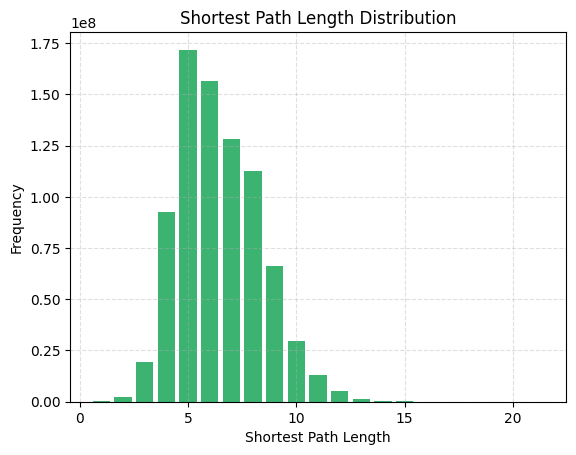
\includegraphics[width=0.6\linewidth]{screenshot001}
	\caption{Shortest path length distribution}
	\label{fig:screenshot001}
\end{figure}
The graph confirms our initial intuition: the shortest path length distribution shows limited variance around the average value, signaling that most of the nodes are reachable in about 3-10 steps. This, again, is a strong clue for the presence of the ``small world'' property. We can easily recover the diameter of the graph
\begin{py}
	diameter = np.max(dist[np.isfinite(dist)])
\end{py}
which is 21. Considering the number of nodes, this is remarkable.
\subsection{Degree analysis}
It is simple enough to obtain the average degree, its standard deviation and the variance. We could compute as $\frac{2L}{N}$, but we can also use the empirical data:
\begin{py}
	#simply use numpy's functions on the list of degrees
	degrees = [deg for _, deg in G.degree()]
	avg_deg = np.mean(degrees)
	std_deg = np.std(degrees)
	var_deg = np.var(degrees)
\end{py}
What we obtain is:
\begin{equation*}
	\ang{k}=6.5593\quad\sigma_{k}=7.9460\quad\var(k)=53.1389.
\end{equation*}
The standard deviation gives us an interesting insight: there is a large variability in the value of the average degree of the network. This suggests us that there hubs there might be present and therefore the degree of the graph may be governed by a power law. By power law, we intend that the probability mass function of the distribution of the degrees can be expressed in the form
\begin{equation*}
	f(k)=ak^{-c}.
\end{equation*}
We can plot the histogram of the degree distribution in figure \ref{fig:screenshot002}.
\begin{figure}[h]
	\centering
	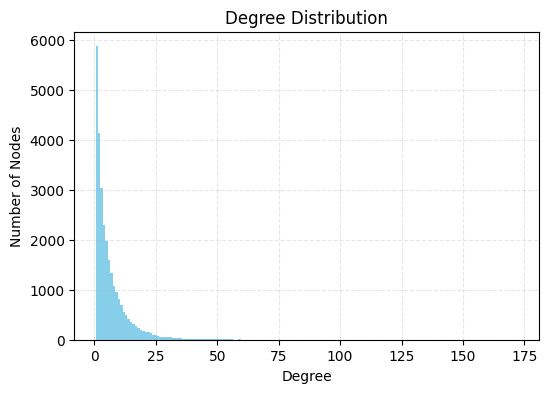
\includegraphics[width=0.6\linewidth]{screenshot002}
	\caption{Degree distribution histogram.}
	\label{fig:screenshot002}
\end{figure}
The shape of the distribution is compatible with the hypothesis of the presence of a power law. We can get a better overview by plotting in figure \ref{fig:screenshot003} the scatterplot of the degree distribution in a $\log-\log$ scale.
\begin{figure}[h]
	\centering
	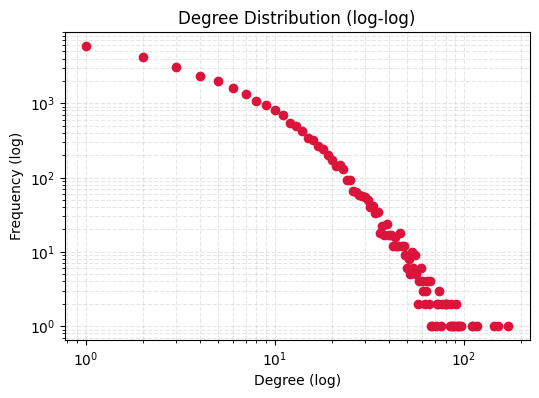
\includegraphics[width=0.6\linewidth]{screenshot003}
	\caption{Scatterplot of the degree distribution}
	\label{fig:screenshot003}
\end{figure}
As we see the degree's trajectory, while retaining the general decreasing profile, is not exactly a straight line as we would expect to see in presence of a graph generated by a power law. From the graph we can infer the presence of ``thin'' tails: in particular, we find more nodes in the ``middle'' part of the spectrum than we would expect in presence of a power law while the probability decays rapidly for higher degree nodes.\par
Using Python's package \pyinl{Powerlaw} we can fit the data to a power law and perform a statistical test to check the $p$-value of the hypotheses:
\begin{equation*}
	\begin{array}{l}
		H_{0}:\text{The power law is not better than the exponential law}\\
		 H_{0}:\text{The power law is better than the exponential law}.
	\end{array}
\end{equation*}
\begin{py}
	#use powerlaw's fitting function
	fit = pw.Fit(degrees, discrete=True)
	print(f"Estimated power-law exponent (alpha): {fit.power_law.alpha:.4f}")
	print(f"Minimum degree for power-law (xmin): {fit.power_law.xmin}")
	
	#compare vs exponential
	R, p = fit.distribution_compare('power_law', 'exponential')
	print(f"Power law vs exponential: R = {R:.4f}, p = {p:.4f}")
\end{py}
The result is:
\begin{center}
	\begin{verbatim}
	Calculating best minimal value for power law fit
	Estimated power-law exponent (alpha): 4.8567
	Minimum degree for power-law (xmin): 45.0
	Power law vs exponential: R = 4.1996, p = 0.2346
\end{verbatim}
\end{center}
The function computes an estimated exponent $c\approx 5$, out of the bounds for a ``scale-free network'' $2<c<3$, but the interesting result is the value found for $x_{\min}$. This means that the minimum degree after which the power law best describes the data is 45; looking at the degree distribution, it is clear that very few nodes overall have a degree $k\geq45$. Moreover, the statistical tests does \textit{not} reject $H_{0}$ neither at the 5\% or at the 10\% confidence level and therefore there is no statistical evidence (according to this test) for the presence of a power law.\par
This may be due to both the platform taken into consideration and the inherent bias of the dataset. For the first matter, it intuitively makes sense that the network doesn't follow a strict power law: while proper social networks like Twitter where anyone can follow anyone and where there exists a clear dynamic of ``rich-gets-richer'', on Deezer (that is ultimately a streaming service) there are no strong incentives in following someone with a large following (to be frank, there is \textit{no} incentive in following anyone). It is reasonable to assume that the social dynamic is fairly different: while it is possible that particularly active users tend to follow other particularly active users, many people may simply follow other people out of interest for their musical library or because they have other relationships outside the platform. Unlike Twitter, where following a large number of people exposes the user to what is ultimately a better (or more intense) fruition of the social network platform, on Deezer this may not be particularly true.\par
The second factor may be in the nature of the data set: who compiled the network chose only \textit{mutual} followers on the platform, thus introducing a bias against all those (directed) edges between non-mutual followers. It is possible that reintroducing this more ``Twitter-like'' dynamic a more strict adherence to a power law would arise.
\subsection{Clustering analysis}
We define the clustering coefficient for node $i$ as 
\begin{equation*}
	C(i)=\frac{2\tau(i)}{k_{i}(k_{i-1})}.
\end{equation*}
This can be interpreted as how likely it is that two nodes, which are both connected to a common third node, are also connected to each other. It is easy to compute it for the whole graph and to plot its results (in figure \ref{fig:screenshot004}):
\begin{py}
	#clustering per node
	clustering = nx.clustering(G)  #returns a dictionary with the node as key and the clustering coefficient as value
\end{py}
\begin{figure}[h]
	\centering
	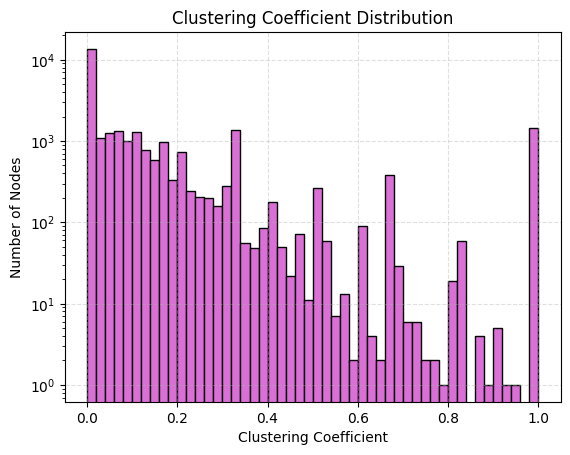
\includegraphics[width=0.6\linewidth]{screenshot004}
	\caption{Clustering coefficient distribution}
	\label{fig:screenshot004}
\end{figure}
The histogram provides interesting insight in how the network behaves. It is clearly not unimodal (in fact, there are two evident spikes at $C(i)=0$ and $C(i)=1$). \par
This suggests that there is a large part of the userbase that tends not to associate in clusters (may be the ``least social-inclined'' fraction of the user-base) while there is a similarly large part of users that is very tightly connected. The latter may be the more active users with respect to the social-networking function, that may tend to form cliques according to musical taste or common listened artists. High clustering might signal the presence of local communities and may help explaining the ``small world'' property that we verified earlier. Moreover, it is interesting to note that the bi-modal nature of the distribution is consistent with the deviation from a pure power law that we supposed earlier.
Another interesting result can be visualized plotting the clustering coefficient against the degree of the nodes:
\begin{py}
	#get degrees and clustering coefficients
	degree_dict = dict(G.degree())
	clustering_dict = nx.clustering(G)
	
	#build arrays for plotting
	degrees = np.array(list(degree_dict.values()))
	clustering = np.array(list(clustering_dict.values()))
\end{py}
The result is visible in figure \ref{fig:screenshot005}.
\begin{figure}[h]
	\centering
	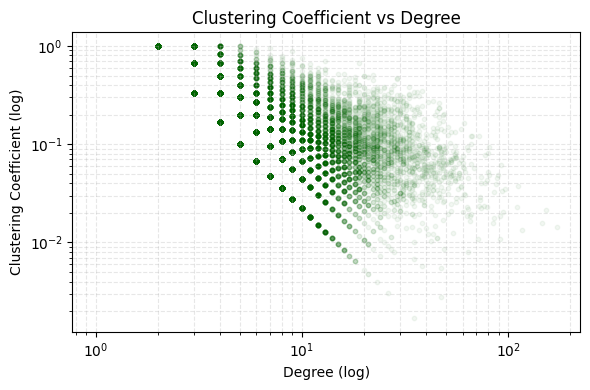
\includegraphics[width=0.6\linewidth]{screenshot005}
	\caption{Scatterplot of clustering coefficient against degree.}
	\label{fig:screenshot005}
\end{figure}
What we see is a general inverse relationship, especially for higher degrees. As the degree of a node increases, its local clustering coefficient tends to decrease. This has the consequence that high-degree nodes (like hubs) tend to have lower local clustering coefficients. Interestingly, this may mean that hubs are not inside cliques or tight communities, but often tend to be points of connection between different communities. This, as said above, may be a result of the fact that users more active on the social networking functions of the site tend to form bridges with a lot of other users regardless of their cluster.\par
Another interesting feature is the fact that as degree increases, the density of points generally decreases, and the spread of clustering coefficient values also seems to narrow towards lower values. The cloud becomes more diffuse and lighter as degree increases, signifying fewer nodes at very high degrees (which corroborates our hypothesis of a law that decays faster than typical power law). \par
To further investigate this question, it can also be interesting to visualize the scatterplot of betweenness against degree. We defined the betweenness of a node as 
\begin{equation*}
	b_{i}=\sum_{h\neq j\neq i}\frac{\sigma_{hj}(i)}{\sigma_{hj}}
\end{equation*}
where $\sigma_{hj}(i)$ is the number shortest paths from $h$ to $j$ passing through $i$ and $\sigma_{hj}$ is the number of shortest paths in general from $h$ to $j$. As for everything involving shortest paths, we use \pyinl{Rustworkx}:
\begin{py}
	betweenness_dict = rx.betweenness_centrality(G_rx)
\end{py}
The result is visible in figure \ref{fig:screenshot006}.
\begin{figure}[h]
	\centering
	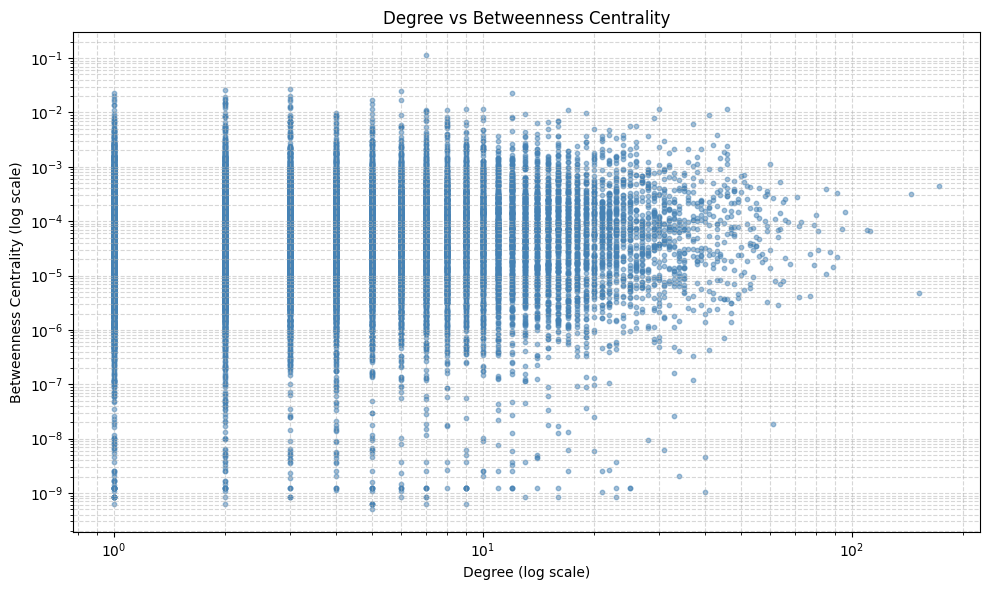
\includegraphics[width=0.6\linewidth]{screenshot006}
	\caption{Scatterplot of betweenness against degree.}
	\label{fig:screenshot006}
\end{figure}
The first most apparent feature of this graph is that nodes with low degrees have wide variability in their betweenness. This suggests the presence of sparse nodes with both high betweenness (possibly bridges between different component of the network) and very low betweenness (possibly peripheral nodes). As degree increases the variability decreases and, surprisingly, so do the maximum values. This is rather counter-intuitive with respect to our previous idea of nodes with high degree being bridges, but since the values tends to concentrate around high-ish betweenness it is not a direct contradiction either. It could indicate the presence of many small, disconnected components, or a very specific growth mechanism that leads to nodes of the same degree having vastly different strategic positions.
\subsection{Largest component}
This is straightforward:
\begin{py}
	#get all connected components (as sets of nodes)
	components = nx.connected_components(G)
	
	#get the largest one (by number of nodes)
	largest_cc = max(components, key=len)
	lcc_size = len(largest_cc)
\end{py}
And the result is... 28281. All nodes are connected, but I believe that this is due to how the network was populated, that is through crawling: starting from a username, the author called the API obtaining the list of mutual followers and for each of this called the API and so on in a recursive manner. By doing this with possibly only one seed it was inevitable that all the components would be connected. This would also account for reachability, by the way.
\subsection{Degree correlation}
It is easy to compute the degree assortativity:
\begin{py}
	#compute assortativity
	assortativity = nx.degree_assortativity_coefficient(G)
\end{py}
We know that a value of assortativity close to 1 indicates assortative structure where high-degree nodes are linked to other high-degree nodes; a value close to -1 indicates disassortative mixing, where high-degree nodes connect to low-degree nodes. In our case the value is 0.1041, indicating mild assortative mixing. This suggests a weak tendency for nodes to connect to other nodes of similar degree. While there's a slight preference for high-degree nodes to connect to other high-degree nodes, and low-degree nodes to connect to low-degree nodes, this preference is not very strong. "birds of a feather flock together" behavior based on how many followers/followed users they have (probably related to the fact that active users are more likely to connect with other active users), it's not the dominant force driving connections. It is also interesting to visualize the plot of the average neighbor degree, that we defined as
\begin{equation*}
	k_{nn}(i)=\frac{1}{k_{i}}\sum_{j}a_{ij}k_{j},
\end{equation*}
 against the node degree in figure \ref{fig:screenshot007}.
\begin{figure}[h]
	\centering
	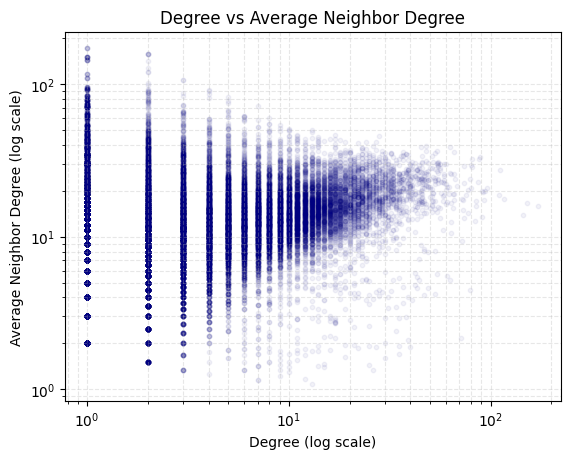
\includegraphics[width=0.6\linewidth]{screenshot007}
	\caption{Scatterplot of average neighbour degree against degree}
	\label{fig:screenshot007}
\end{figure}
As for the previous plot, low degrees show very high variance: there is a strong heterogeneity in how nodes of the same degree connect. However, as degree increases, these bands start to merge into a more diffuse cloud. Overall, the plot corroborates the low positive assortativity: high degrees do tend to associate with high degrees neighbors, but only slightly. This relative neutrality in degree mixing adds to the picture of a social network that, while connected and having communities, deviates from the idealized "scale-free" model with strong degree-based homophily. Other factors, such as shared musical tastes or existing real-world friendships, likely play a more significant role in connection formation than solely the number of existing connections.
\subsection{Communities}
In a wide network like the one that we are discussing, basic \pyinl{Networkx} functions are not fast enough. Since \pyinl{Rustwork} does not implement (yet) clustering algorithms, we will use \pyinl{Igraph}'s clustering capabilities. We start by calculating communities using Louvain's algorithm:
\begin{py}
	G_ig = ig.Graph.TupleList(G.edges(), directed=False)
	partition = G_ig.community_multilevel()  #louvain
\end{py}
This algorithm detects 94 communities and the resulting graph can be visualized in figure \ref{fig:screenshot008}. 
\begin{figure}[h]
	\centering
	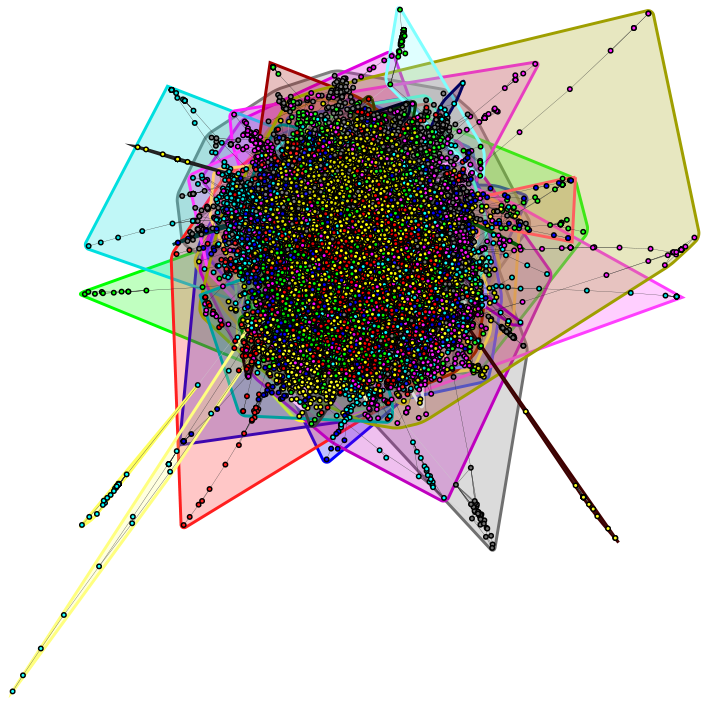
\includegraphics[width=0.6\linewidth]{screenshot008}
	\caption{Result of the Louvain algorithm with maximum resolution.}
	\label{fig:screenshot008}
\end{figure}
Of course, this visualization is not very helpful. We can print some basic statistics:
\begin{py}
	community_sizes = [len(c) for c in partition]
	
	#print some basic information
	sizes = np.array(community_sizes)
	print(f"Number of communities: {len(sizes)}")
	print(f"Modularity of the partition: {partition.modularity:.4f}")
	print(f"Min size: {sizes.min()}")
	print(f"Max size: {sizes.max()}")
	print(f"Mean size: {sizes.mean():.2f}")
	print(f"Median size: {np.median(sizes):.2f}")
	print(f"Std dev: {sizes.std():.2f}")
\end{py}
which gives
\begin{center}
	\begin{verbatim}
					Number of communities: 81
					Modularity of the partition: 0.6838
					Min size: 4
					Max size: 4556
					Mean size: 349.15
					Median size: 31.00
					Std dev: 742.40
	\end{verbatim}
\end{center}
The high value in modularity seems to confirm that the Louvain algorithm managed to optimize this quantity enough and it may signal a significant and well-defined community structure.\par
The median size is much lower than the mean size and it strongly indicates a highly skewed distribution of community sizes. This is confirmed by the histogram of the distribution of community sizes in \ref{fig:screenshot009}: there are many small communities, which pull the median down, while a few very large communities significantly inflate the mean.
\begin{figure}[h]
	\centering
	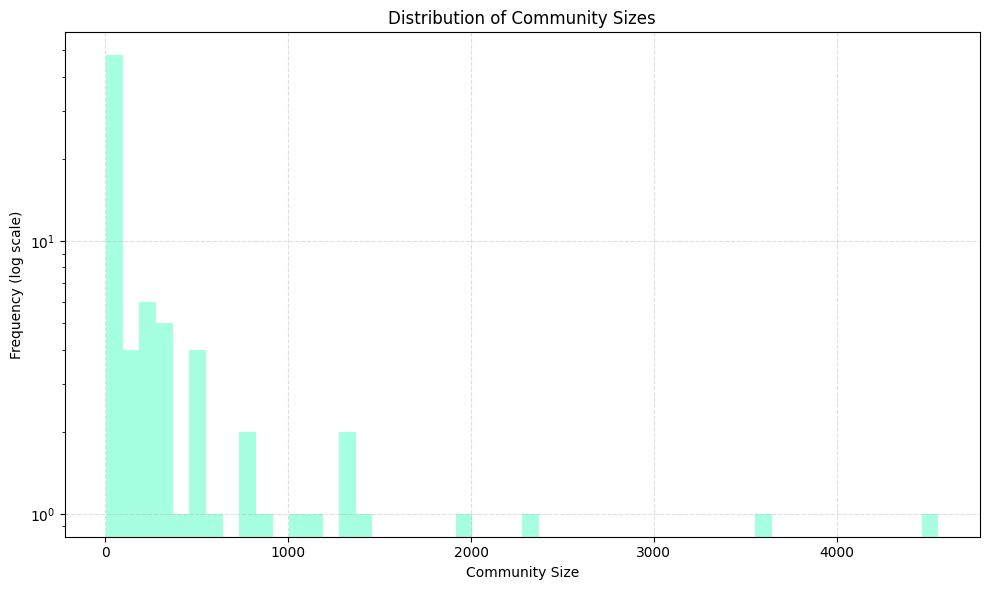
\includegraphics[width=0.6\linewidth]{screenshot009}
	\caption{Histogram of community sizes}
	\label{fig:screenshot009}
\end{figure}
The histogram confirms that the majority of the 81 detected communities are relatively small. These likely represent tightly-knit groups of friends, niche music fan bases, or very specific social circles on Deezer. This aligns with the peak at high clustering coefficients we observed earlier.\par
While most communities are small, there are a few very substantial communities that likely form the backbone or broader social contexts within the Deezer network. These larger communities might comprise users with broader interests or act as bridges between smaller, more specialized groups.\par
To visualize how the communities and their modularities interact with each other, we can plot the intra-community degree $k_{\mathrm{in}}$ against the infra-community degree $k_{\mathrm{out}}$: 
\begin{py}
	#create a map node -> community
	membership = partition.membership
	node2comm = {v.index: membership[i] for i, v in enumerate(G_ig.vs)}
	
	internal_deg = []
	external_deg = []
	
	for v in G_ig.vs:
		comm = node2comm[v.index]
		deg = G_ig.degree(v.index)
		internal = 0
		for neighbor in G_ig.neighbors(v.index):
			if node2comm[neighbor] == comm:
				internal += 1
		external = deg - internal
		internal_deg.append(internal)
		external_deg.append(external)
\end{py}
\begin{figure}[h]
	\centering
	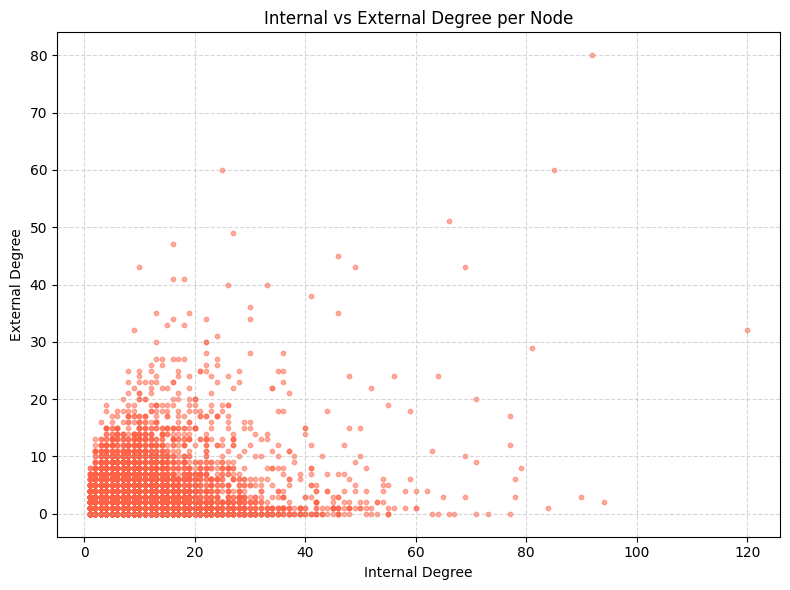
\includegraphics[width=0.6\linewidth]{screenshot010}
	\caption{Scatterplot of $k_{\mathrm{in}}$ against $k_{\mathrm{out}}$.}
	\label{fig:screenshot010}
\end{figure}
The resulting plot is Figure \ref{fig:screenshot010}. The most concentrated area of points is in the bottom-left corner, at very low internal and external degrees ($k_{\mathrm{in}}<10$ and $k_{\mathrm{out}}<10$). As we move along the $x$ axis and the higher internal degree of the community increases, we also register a high spread on the $y$ axis reaching around the value of 80 for $k_{\mathrm{out}}$. This means that, among strongly internally connected communities, some of them still have mostly internal connections but (a few) others have a high out-degree, making them bridges between different communities.  The existence of this pattern is precisely what we would expect in a network with high modularity: the communities are well-defined, so most connections are internal, but some connections must be external to link the communities together.  The scatter of points, without a very tight grouping or strong diagonal trend, is also consistent with weak assortativity. It suggests that the formation of internal and external ties is not rigidly determined by the overall degree of nodes in an assortative manner.\par
To compare this result with another feasible clustering algorithm we can perform analogous operations with a label propagation algorithm. The basic statistics are:
\begin{center}
	\begin{verbatim}
					Number of communities: 1984
					Modularity of the partition: 0.4888
					Min size: 2
					Max size: 13494
					Mean size: 14.25
					Median size: 3.00
					Std dev: 305.65
	\end{verbatim}
\end{center}
The number of communities is extremely higher than the one obtained by the Louvain algorithm. The modularity score is lower, but this is expected since the Louvain algorithm explicitly optimizes for modularity; however, the score is still rather high. The histogram is not particularly helpful, as we can see in figure \ref{fig:screenshot011}. The vast majority of communities has a very low size, except for some rare cases and a notable outlier towards the maximum size of 13494 (almost half of the network!).
\begin{figure}[h]
	\centering
	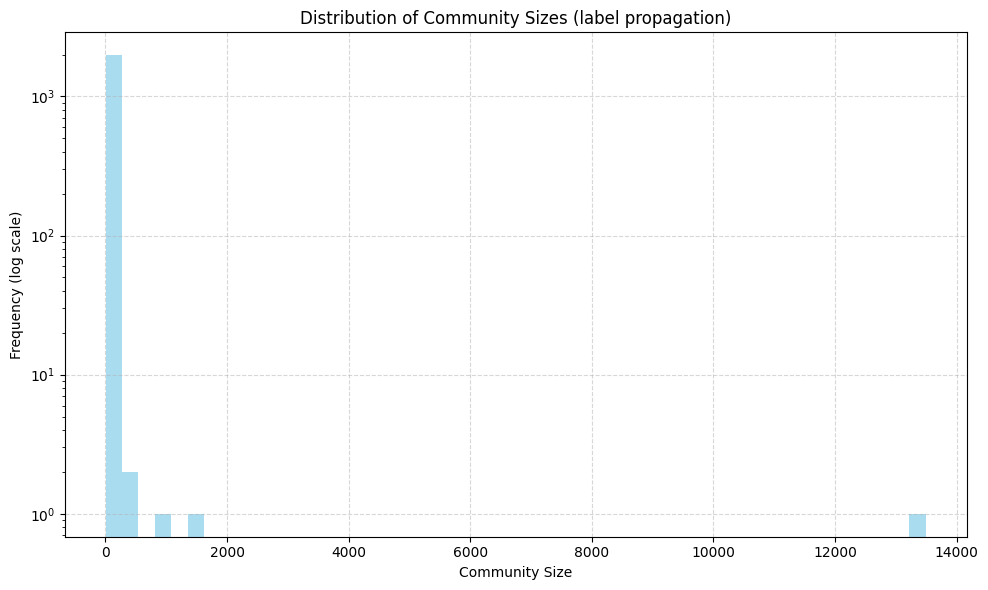
\includegraphics[width=0.6\linewidth]{screenshot011}
	\caption{Histogram of distribution of community sizes with label propagation}
	\label{fig:screenshot011}
\end{figure}
The Louvain method seems more solid and it appears to bear more significance with respect to community detection.
\subsection{Centrality measures}
We can start by analyzing the closeness measure of the nodes in the network. We defined centrality as
\begin{equation*}
	g_{i}=\frac{1}{\sum_{j\neq i}\ell_{ij}}
\end{equation*}
where $\ell_{ij}$ is the distance between nodes $i$ and $j$. This is an important centrality measure that assesses how ``close'' a node is to all other nodes in the network. Since closeness involves shortest paths, we need to use \pyinl{Rustworkx} once again:
\begin{py}
	closeness = rx.closeness_centrality(G_rx)  #returns a dict: node -> closeness
	closeness_values = list(closeness.values())
\end{py}
The results are plotted in the histogram in Figure \ref{fig:screenshot012}.
\begin{figure}[h]
	\centering
	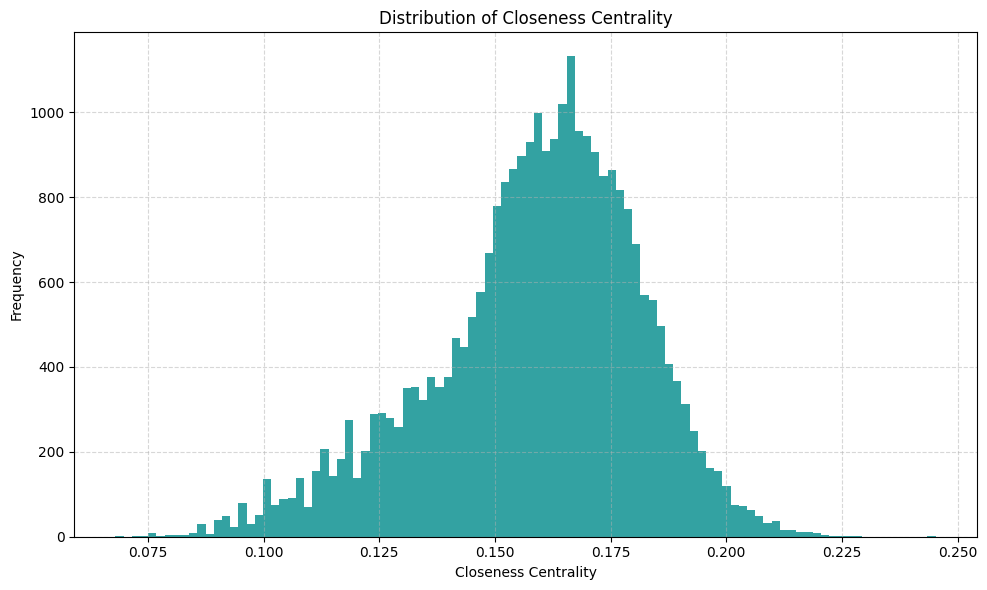
\includegraphics[width=0.6\linewidth]{screenshot012}
	\caption{Histogram of closeness centrality.}
	\label{fig:screenshot012}
\end{figure}
This distribution has an interestingly bell-shaped distribution peaking around 0.165 to 0.175. This suggests that the majority of nodes have a similar ``closeness'' to all other nodes in the network. There's a high concentration of nodes around the peak, with frequencies dropping off symmetrically on either side. This implies that most nodes are ``average'' in terms of how quickly they can reach other nodes. Most nodes are efficient at reaching other nodes and this, together with the small average distance, makes a point in favor of the ``small world'' property. Moreover, it seems like there is no dominant central core with excessively high centrality.
\begin{figure}[h]
	\centering
	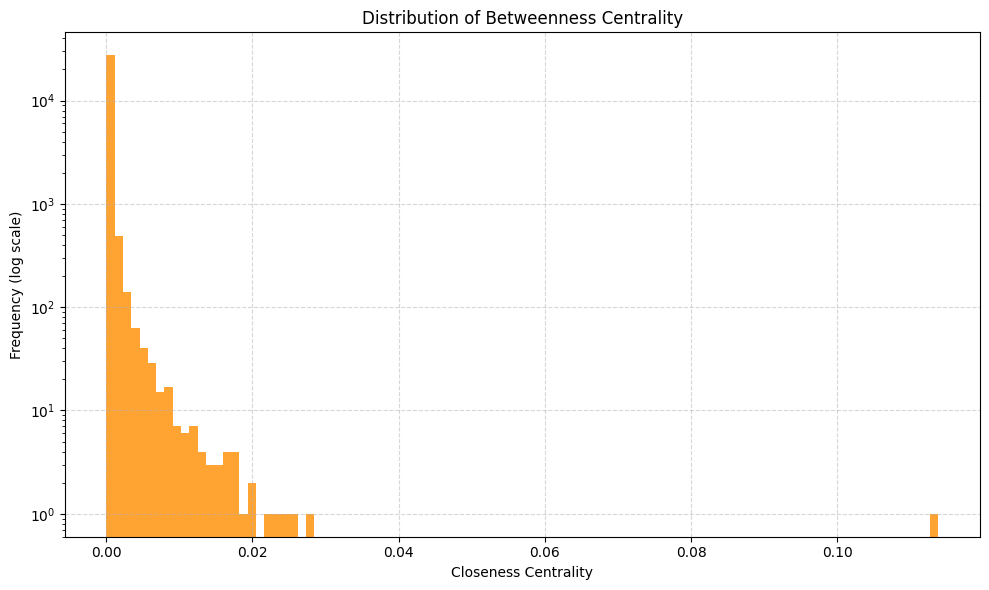
\includegraphics[width=0.6\linewidth]{screenshot013}
	\caption{Histogram of betweenness centrality}
	\label{fig:screenshot013}
\end{figure}
An interesting insight comes from the histogram of betweenness centrality in figure \ref{fig:screenshot013}.
The histogram shows a very sharp and tall peak at extremely low betweenness centrality values, very close to 0 (around 0.00-0.0025). This indicates that the vast majority of nodes in your network have very low betweenness centrality. They don't lie on many shortest paths between other pairs of nodes. This means that while the vast majority of users have very little control over information flow via shortest paths, a small number of ``bridge'' users are critically positioned to connect disparate parts of the network. Again, we find a quite vaporous clue of the existence of these ``bridge'' nodes.
\begin{figure}[h]
	\centering
	
\includegraphics[width=0.6\linewidth]{screenshot014}
	\caption{Cumulative distribution function for betweenness centrality}
	\label{fig:screenshot014}
\end{figure}
The plot in figure \ref{fig:screenshot014} can shed a different light on the subject. It is the plot of the distribution's cumulative distribution function
\begin{equation*}
	\pr(B_{i}\geq b_{i})
\end{equation*}
for the beetweenness measure. First of all, it is another confirmation that the network is \textit{not} governed by a power law, since its CDF on the log-log graph would be a straight line. The curve starts very low on the $y$ axis and then rises sharply in the extremely low betweenness centrality range (from $10^{-9}$ to $10^{-7}$). This indicates that a vast majority of nodes have very low betweenness centrality.\par
Another interesting metric is the heterogeneity parameter $\kappa$:
\begin{equation*}
	\kappa=\frac{\ang{k^{2}}}{\ang{k}^{2}}
\end{equation*}
with
\begin{equation*}
	\ang{k}=\frac{\sum_{i}k_{i}}{N}\qquad\ang{k^{2}}=\frac{\sum_{i}k^{2}_{i}}{N}.
\end{equation*}
This is straightforward to compute:
\begin{py}
	degrees = [deg for _, deg in G.degree()]
	kappa = np.mean([k**2 for k in degrees]) / (np.mean(degrees))**2
\end{py}
and the value is 2.4675. A $\kappa$ value close to 1.0 would indicate a homogeneous network (like a random Erdos-Renyi graph) where most nodes have degrees close to the average. The value that we obtained suggests that the network is actually heterogeneous. This means there is a noticeable disparity in node degrees, with a substantial number of low-degree nodes and a smaller but significant number of higher-degree nodes (possibly hubs). The high heterogeneity in betweenness distribution is also coherent with a high general heterogeneity parameter.\par
At this point, we incur in a little contradiction: it looks like the closeness centrality measure is at odds with the heterogeneity parameter $\kappa$ and the betweenness centrality. In a small-world network, even if a few hubs or bridges exist (leading to degree and betweenness heterogeneity), the overall connectivity is so efficient that most nodes are just a few steps away from each other. This high overall efficiency means that the distance to any other node doesn't vary wildly for most nodes, leading to a more concentrated closeness centrality distribution.
\subsection{Homophily}
The data set comes with an additional file specifying the gender of each node, so we can perform homophily detection on that set. We start by assigning attributes from the CSV to the nodes:
\begin{py}
	#load the CSV
	gender_csv = pd.read_csv("deezer_europe_target.csv")
	#create a dict {node_id: gender}
	gender_dict = pd.Series(gender_csv["target"].values, index=gender_csv["id"]).to_dict()
	#set attribute to nodes
	nx.set_node_attributes(G, gender_dict, name="gender")
\end{py}
We said that there is signal of homophily between two groups $A$ and $B$ if $p$ is the fractions of nodes in $A$ and $q$ in $B$ then we have homophily if \begin{equation*}
	\#\text{ of cross groups edges }<2pq.
\end{equation*}
We compute the necessary quantities and then we print the result:
\begin{py}
	#computations for homophily
	same = 0
	diff = 0
	#computing cross rations
	for u, v in G.edges():
		gu = G.nodes[u].get("gender")
		gv = G.nodes[v].get("gender")
		if gu == gv:
			same += 1
		else:
			diff += 1
	
	total = same + diff
	observed_cross_ratio = diff / total
	
	#compute expected cross-gender edge fraction
	genders = [G.nodes[n].get("gender") for n in G.nodes() if "gender" in G.nodes[n]]
	freqs = cl.Counter(genders)
	n_total = sum(freqs.values())
	p = freqs[0] / n_total
	q = freqs[1] / n_total
	expected_cross_ratio = 2 * p * q
	
	print(f"Observed cross-gender edge ratio: {observed_cross_ratio:.4f}")
	print(f"Expected cross-gender ratio (random mixing): {expected_cross_ratio:.4f}")
	
	if observed_cross_ratio < expected_cross_ratio:
		print("Evidence of homophily: fewer cross-gender edges than expected.")
	else:
		print("No homophily detected.")
\end{py}
The result is:
\begin{center}
	\begin{verbatim}
					Observed cross-gender edge ratio: 0.4749
					Expected cross-gender ratio (random mixing): 0.4936
					Evidence of homophily: fewer cross-gender edges than expected.
	\end{verbatim}
\end{center}
The difference between the observed and expected ratio (0.4936 - 0.4749 = 0.0187 or about 1.87 percentage points) is relatively small. This indicates that while homophily exists, it's not an extremely strong effect. It's not the case that male users only connect with other male users, or vice versa; there's still a large proportion of cross-gender connections.\par
\section{Comparison with random models}
To assess the qualities of a network it is important to compare it with ``planted'' networks that we know present determinate characteristics. First of all, we produce our random networks according to four models:
\begin{enumerate}
	\item Erdős-Rényi model (random graph);
	\item Watts-Strogatz model;
	\item Configuration Model (degree-preserving);
	\item Barabási-Albert (preferential attachment).
\end{enumerate}
\begin{py}
	N = G.number_of_nodes()
	L = G.number_of_edges()
	avg_degree_real = 2 * L / N
	
	#1)Erdős-Rényi (ER)
	p_er = avg_degree_real / (N - 1)
	G_er = nx.erdos_renyi_graph(N, p_er, seed=123)
	
	#2)Watts-Strogatz (WS)
	n_neigh = int(round(avg_degree_real))
	if n_neigh % 2 != 0:  # must be even
		n_neigh += 1
	p_shortcut = 0.1
	G_ws = nx.watts_strogatz_graph(N, n_neigh, p_shortcut, seed=123)
	
	#3)Configuration Model (degree-preserving)
	degree_seq = [deg for _, deg in G.degree()]
	G_conf = nx.configuration_model(degree_seq, seed=123)
	G_conf = nx.Graph(G_conf)  #simplify graph (remove parallel edges)
	G_conf.remove_edges_from(nx.selfloop_edges(G_conf))
	
	#4)Barabási-Albert (BA)
	m = max(1, int(round(avg_degree_real / 2)))
	G_ba = nx.barabasi_albert_graph(N, m, seed=123)
\end{py}
Here:
\begin{itemize}
	\item the ER model is straightforwardly initliazed with the same number of nodes and as probability the average degree $\ang{k}$;
	\item the WS model is initliazed with a probability of "shortcut" equal to an arbitrary $0.5$;
	\item the CFG model has the same sequence of degrees as the actual network;
	\item in the BA model each new node brings in $m$ new edges so the total number of edges $\approx m \times (n - m_{0})$ which is approximately $m\times n$ for large $n$. That means the average degree is $\approx 2m$.
\end{itemize}
We create a function to provide a general overview of the networks:
\begin{py}
	def analyze_graph(G, name):
	
	N = G.number_of_nodes()
	L = G.number_of_edges()
	avg_deg = 2 * L / N
	clustering = nx.average_clustering(G)
	assortativity = nx.degree_assortativity_coefficient(G)
	
	if nx.is_connected(G):
	#convert to rx graph
	G_rx = rx.networkx_converter(G)
	else:
	Gcc = G.subgraph(max(nx.connected_components(G), key=len)).copy()
	G_rx = rx.networkx_converter(Gcc)
	
	avg_path_len = rx.unweighted_average_shortest_path_length(G_rx)
	
	print(f"--- {name} ---")
	print(f"Nodes: {N}")
	print(f"Edges: {L}")
	print(f"Average Degree: {avg_deg:.4f}")
	print(f"Average Clustering: {clustering:.4f}")
	print(f"Average Path Length: {avg_path_len:.4f}")
	print(f"Degree Assortativity: {assortativity:.4f}")
	print()
\end{py}
The results of the run are summarized in table 1.
\begin{table}[h!]
	\centering
	\label{tab:network_comparison}
	\begin{tabular}{|l|c|c|c|c|c|}
		\hline
		\textbf{Property} & \textbf{Network} & \textbf{ER} & \textbf{WS} & \textbf{BA} & \textbf{Cfg} \\
		\hline
		Average degree & 6.5593 & 6.5456 & 8.0000 & 5.9994 & 6.5541 \\
		Average clustering & 0.1412 & 0.0002 & 0.0832 & 0.0022 & 0.0009 \\
		Average path length & 6.4498 & 5.6749 & 5.4862 & 4.6372 & 4.8591 \\
		Degree assortativity & 0.1041 & -0.0055 & -0.0410 & -0.0245 & -0.0024 \\
		\hline
	\end{tabular}
	\caption{Comparison of actual network against random networks}
\end{table}
Some observations:
\begin{itemize}
	\item \textit{average degree}: WS and BA models have slightly different edge counts/average degrees, which is normal given their construction mechanisms. This ensures a fair comparison for other properties;
	\item \textit{average clustering coeffcient}: ER, BA and CFG exhibit extremely low clustering. This is expected, as they are primarily random or growth models that don't explicitly promote local triadic closure. Our real network is much more locally dense. The WS tands out with a much higher clustering coefficient than the real network. This is by design, as WS is specifically built to have high clustering (like regular lattices) while maintaining short path lengths. This suggests that while Deezer is locally clustered, it's not as highly clustered as a WS small-world network, or perhaps has a more varied local structure;
	\item \textit{average path length}: all the random networks exhibit shorter path lengths;
	\item \textit{degree assortativity}: all the random networks exhibit near-zero or slightly negative (disassortative) assortativity. This is a critical difference. Random networks typically show no preference for degree-based mixing, while scale-free networks (like BA) are often disassortative (hubs prefer connecting to low-degree nodes). The positive assortativity of the real network sets it apart from these models, identifying it as a more ``social network''-like structure in terms of degree mixing.
\end{itemize}
Another interesting point of comparison lies in the different graphs for the log-log degree probability.
\begin{py}
	def plot_degree_distribution(graphs, title="Degree Distribution (log-log)"):
		plt.figure(figsize=(10, 6))
		
		for name, G in graphs.items():
			degrees = [d for _, d in G.degree()]
			degree_counts = np.bincount(degrees)
			#trim zero values
			degrees_nonzero = np.nonzero(degree_counts)[0]
			counts_nonzero = degree_counts[degrees_nonzero]
			
			#normalize to probability
			prob = counts_nonzero / counts_nonzero.sum()
			
			plt.plot(degrees_nonzero, prob, marker='o', linestyle='-', label=name)
		
		plt.xscale('log')
		plt.yscale('log')
		plt.xlabel("Degree (log scale)")
		plt.ylabel("Probability (log scale)")
		plt.title(title)
		plt.legend()
		plt.grid(True, which="both", ls="--", alpha=0.5)
		plt.show()
\end{py}
\begin{figure}[h]
	\centering
	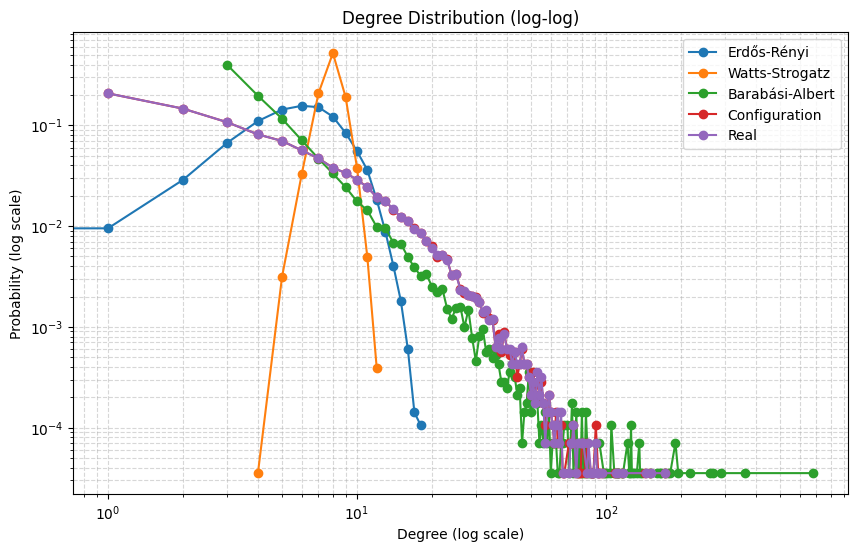
\includegraphics[width=0.6\linewidth]{screenshot015}
	\caption{Summary of all degree distributions.}
	\label{fig:screenshot015}
\end{figure}
The result is plotted in Figure \ref{fig:screenshot015}. Here we can see that the BA model has exactly the shape that we would expect from a network equivalent to our real one but with power law. Again, we can see how our degree distribution deviates from it. The CFG plot is, of course, identical to the real one. WS and ER have a radically different degree distribution.\par
Another interesting visualization in Figure \ref{fig:screenshot016} is the so-called clustering spectrum, that is the average clustering coefficient as a function of the degree. Here:
\begin{figure}[h]
	\centering
	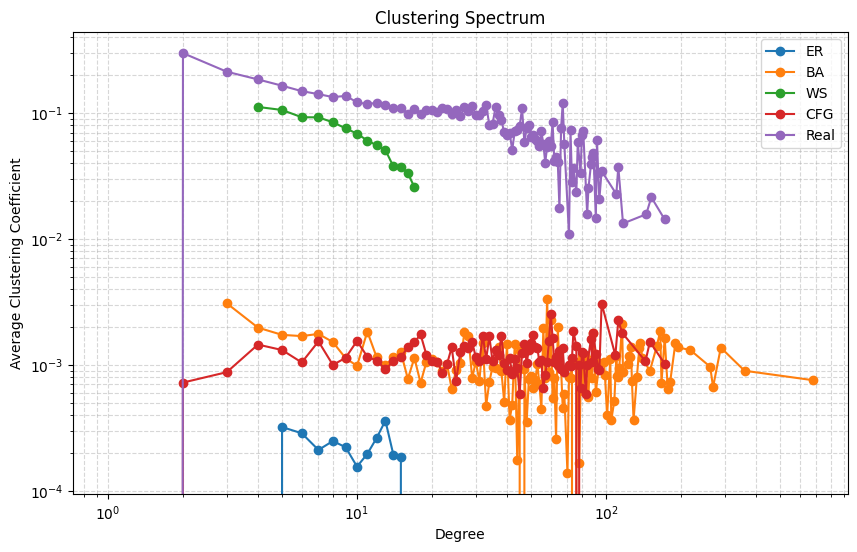
\includegraphics[width=0.6\linewidth]{screenshot016}
	\caption{Clustering spectrum of the networks}
	\label{fig:screenshot016}
\end{figure}
\begin{itemize}
	\item \textit{real network}: the real network demonstrates a characteristic decreasing trend in average clustering coefficient with increasing degree. Nodes with very low degrees exhibit relatively high clustering values (around 0.4-0.5). As degree increases, the clustering coeffcient systematically drops, reaching values around 0.01-0.02 for high-degree nodes. In this case, highly connected nodes (possibly hubs) find it increasingly difficult for all their numerous neighbors to be interconnected;
	\item \textit{ER}: the ER i model exhibits extremely low average clustering coefficients across all degrees. This is expected, as connections in an ER random graph are formed purely by chance, which rarely results in the formation of local triangles. The ER line is significantly lower than the "Real" network's line for all degrees;
	\item \textit{WS}: the WS model (at its specific parametrization) begins with remarkably high clustering coefficients for low degrees (near 1.0), a direct carryover from its initial regular lattice structure. It then shows a decreasing trend with increasing degree, but it generally maintains higher clustering values than the real network for its observed degree range. Of course, this model has the ``small world'' property;
	\item \textit{CFG}: the CFG model displays extremely low average clustering coefficients across all degrees, mirroring the values of other purely random models (like ER and BA).
\end{itemize}
\section{Conclusions}
In this brief discussion we have analyzed the social network of some European users of the music streaming platform Deezer. We have seen how the network shows peculiar and irregular characteristic that do not exactly fit into the cases that we have seen during our course. In general, while retaining a strong and evident ``small world'' property, the network didn't align with any power law hypothesis. Further analysis has brought new light over the particular structure of ``quiet'' hubs and assortativity while the comparison against the principal models of random graphs has remarked the differences between our real network and the theoretical counterparts.
\end{document}
